% This example An LaTeX document showing how to use the l3proj class to
% write your report. Use pdflatex and bibtex to process the file, creating 
% a PDF file as output (there is no need to use dvips when using pdflatex).

% Modified 

\documentclass{l3proj}
\usepackage{graphicx}

\setlength{\parindent}{5ex}
\begin{document}

\title{Nutriplotter}

\author{Han Loo, 2288527\\
        Eleonora Della, 2244079\\
        Soma Froghyar, 2267217\\
        Matthew Smith, 2260469\\
        Peter Macaldowie, 2258785}

\date{23 March 2019}

\maketitle

\begin{abstract}

The game application developed for our client - the School of Medicine, Dentistry and Nursing - allows for the creation of a complete and balanced meal virtually. The task given was to implement a plate model which would be suitably dynamic in order to allow for balancing of its components, leading to a balanced meal according to the UK National Guidelines.\par
Throughout the project, the team made the decision to use Expo and Firebase as their main technologies. Agile project management was utilised throughout the whole project to aid the software development process. The aim of this report is to discuss the considerations we have taken as a team and the practices we have adopted in order to successfully produce the required deliverables for our client, as well as some of the learning outcomes that resulted from the software development process.\par
\end{abstract}

%% Comment out this line if you do not wish to give consent for your
%% work to be distributed in electronic format.
\educationalconsent

\newpage

%==============================================================================
\section{Introduction}
The following document presents Team SE04's group project. The project involved developing a mobile application which had as a main goal the creation of a balanced meal. Working alongside the School of Medicine, Dentistry and Nursing, our main goal was to educate people about the National Nutrition Guidelines by providing them with an interactive user interface which would help them create their plate and adjust its components accordingly to make it balanced. \par
Our team consisted of five Software Engineering students from the University of Glasgow. Our dissertation aims to provide an overview of our journey from researching to the process of developing the actual software and finally producing the final product. By adopting the methods outlined in our dissertation, we were able to successfully deliver the product to our client, to a degree with which the client seemed pleased with.\par
The School of Medicine, Dentistry and Nursing challenged us to develop a mobile application for both Android and iOS devices. The application was to be successfully built and run with both operating systems while also interacting with a database. This task led to our project being developed and functioning with two main platforms, Expo and Firebase. Those platforms were used in order to get a fully functioning application which could retrieve from a database while having a competent user interaction.\par

%% Final paragraph.
The structure of the rest of this report is as follows; Section 2 gives background information on the actual project, its context and aims of the project as a whole, as well as the customer. The main sections of the report, from section 3 through 8, assess each point in our software development, portraying the achievements we earned as a team and the learning outcomes that resulted when attempting different development methods and practices. Concluding with section 9, we give an overview of our success, and the knowledge that we have gained both as individuals and also as a team which we will be able to implement in future projects moving forward.\par
%==============================================================================
\section{Case Study Background}
\label{case study background}
\subsection{Customer Background}
The School of Medicine, Dentistry and Nursing of the University of Glasgow is one of the largest Undergraduate schools in the United Kingdom. The primary purposes of the school involve providing training and experience to medical students and the conduction of research surrounding the topics denoted in the school's full title. They provide medical training to students who are highly sought after following graduation, due to the school's international reputation. They particularly pride themselves on their capability to give students suitable teaching to leave them suitably equipped for a career in Medicine in the 21st century. \par
Our primary client is the Chair of Human Nutrition, although we liaised with another member of the school for some time before meeting the client, due to their busy schedule. The research interests of our primary client encompass the wide range of molecular, clinical and public health aspects of Human Nutrition, a body of integrated sciences underpinning all biomedical and health research. \par
\subsection{Project Background}
Although several ‘healthy eating' apps currently exist; two major challenges remain: saturation of the provision of fact-based nutritional information and encouraging regular use of the app to ensure continued changes in eating choices. Additionally, the apps can often expect users to completely change the way they eat by providing meal plans from the first usage. This is simply not realistic for many users, something which our client explained before proposing their solution, which was initially conceived years ago by them. \par
The app we were to build would deliver nutrition education via a tool in which users create a meal on a ‘digital plate' from a selection of food choices. The aim of the tool was to create and present a nutritionally balanced meal, in accordance with the ‘Balanced Plate' model, which the client drew our attention to. The app would engage users in a fun and informative manner and help to provide them with the ability to make their own nutritionally balanced choices, while not immediately forcing them to entirely change their diet. Instead, the aim of the proposal was to help users make informed decisions according to their own diet, with suggestions of how a plate might be improved nutritionally to be more balanced.\par
%==============================================================================
\section{Requirements Gathering}
\label{sec:requirements gathering}
Although our team had minor complications during the requirement gathering process, the outcome was rewarding. Following our first meeting, it was easy to begin developing our requirements documentation through the use of user stories and personas. Our project had a very broad user base, aiming to cater to a wide variety of users from many backgrounds. Having identified the user base, we were able to delve further into the finer details of these 'personas', allowing us to develop a clear idea of the users' goal.\par
The project specifications provided initially to the team were somewhat unclear, meaning that further clarification was required in future meetings. The client required that we make the balanced plate model the central focus of the app, unlike generic health apps in the market. Once this clarification was made, development could begin using the amended specifications.\par
Our client suggested that we create a survey based on eating habits. Our presentation of our researching findings alongside the survey results gave the client a better understanding on technology options, existing and similar applications in the market. In return, this aided our requirements gathering process tremendously. \par
\subsection{User Stories}
User stories were used primarily to document practical information of what the user aimed to gain when using our app. User stories are written so that each can be given an estimate of how difficult or time–consuming it will be to develop, allowing for better prioritisation of tasks. This mitigated the time consumed discussing features of application, as it allowed us to address a user-driven approach for several of the perceived challenges in quick succession. Story mapping enhanced the team's shared understanding of each feature, and was conducted by connecting the elements denoted in user stories to the features and the overall product roadmap. This helped in areas of estimating and scheduling the order of tasks of the project.\par
We believe that user stories were crucial to the success of our requirements by aiding transparency, improving collaboration, creating shared understanding and orienting the teams to focus on customer needs. The benefits gleaned from it helped to eliminate various potential risks and misconceptions, which largely arose from both communication and technical issues.\par
%==============================================================================
\section{Customer Interaction}
\label{sec: customer interaction}
\subsection{Slack and Customer Interaction}
\label{slack and customer interaction}
Involving the customer when it comes to a software development process improves the chances that the final product will meet the requirements and perform well according to the customers' needs. Thus, our team made sure that customer interaction played a vital role within the project. This involved weekly communication with the customer, as well as our interactions with them on the customer demonstration days. From the very first meeting we had with the customer, various topics had been discussed including gathering of early requirements and getting more insight concerning the project, but one of the key discussion topics was how we would communicate with the customer. After the first meeting we decided on using Slack for communicating and arranging meetings together with the customer.\par
Slack was successfully set up from the first week of starting the project, however, we were unsuccessful on using Slack as much as we planned to. By giving more thought into this, we identified that the main reason was that our main discussion was happening through Messenger group chat that we had as a team. Although our main platform for communication wasn't Slack, we did use it to arrange fortnightly meetings with the customer as well as inform the customer for any important updates on the development of our application.\par
\subsection{Early Contact Issues}
\label{early contact issues}
At first, communicating with our client was a bit challenging due to dealing with setting up Slack for everyone and getting familiar with it. After everything had been set up successfully and everyone was subscribed to the right channel, we were able to exchange important documents with the client that would help us further in our research and plan our second meeting successfully. \par
After our first customer demonstration day, we asked to meet with the person who had the idea for the mobile application so we can get the answers we required, as we felt we were headed in the wrong direction. On the 27th of November we met with the idea originator who successfully answered our questions. Although his idea didn't match what we had so far, we now knew what we were supposed to do and started working towards implementing the altered application. Reflecting on this, we believe we should have made contact with the idea originator in the early stages which would have helped us head into the right path from the beginning. \par
\subsection{Customer Demonstrations}
\label{subsec:customer demonstrations}
From the moment we were given the project, to the day we handed the customer our finished product, we had five customer demonstration days planned and completed successfully. 
After our first meeting, our task was to do research on other existing applications and gather all information required to start developing, including carrying out planning poker and creating wireframes. \par
When our first customer demonstration was done, we were very pleased with the progress we had done so far as we also had a demo to show together with our research findings. The client was quite happy with what we had presented, although, it was pointed out that we might be heading the wrong way with the idea and it would be best to arrange a meeting with the idea originator to explain in detail his vision about the mobile application. \par
Between the first demonstration and the second demonstration, a meeting with the idea originator was arranged which changed our original plans and wireframes, as well as making us start over with the development. This was a slight diversion from our original plans but we acted quickly and were able to produce a demo for our second demonstration. For every customer demonstration we prepared a set of questions that would help us understand whether we were succeeding in meeting the customer's expectations. Both the questions and responses to the application were used as our main source of feedback from the customer demonstration meetings and they helped us greatly in figuring out how to proceed next. At the end of every meeting, we concluded by agreeing to a set of goals for the next iteration. Having this in mind we were able to split up the tasks responsibly to produce a fair amount of work for each sprint.\par
Reflecting on customer interaction, as we began digging deeper into the project our communication greatly improved. At the beginning, due to having to set up Slack and not having communication with the idea originator, we were held back a bit but once this was resolved and we were underway, we were improving the customer communication weekly as well as our project development. Considering the demonstration days that took place, we realised that as time went on these improved as well. Initially we were a bit lost on how to present our progress, and what to expect from these meetings but once we got our first one done we felt more confident in knowing how to prepare for them. Overall, we believe that we kept our interaction with the customer very constructive and balanced during the whole process.

%==============================================================================
\section{Software Process Practices}
\label{sec:software process practices}
\subsection{Retrospectives}
\label{subsec: retrospectives}
A retrospective is a meeting that's held at the end of an iteration in Agile software development. During the retrospective, the team reflects on what happened in the iteration and identifies actions for improvement going forward. These retrospectives enable the team to make small improvements regularly, and apply them in a controlled and immediate manner. The goal of retrospectives is helping teams to improve their engineering process. Our retrospective used the liked, lacked, longed for method. This is conducted by giving each member a pen and several post it notes stating what they liked about the project during the last iteration, lacked during the last iteration and longed for in the next sprint of the project. Individual responses were attached on a board and group members would discuss each one. Our coach was present during each retrospective to provide further comments if necessary. \par
A retrospective was conducted after each customer meeting, marking the end of the current iteration. This allowed for team members to look back, present their views and share their experiences effectively. Retrospective provided the medium to consider the factors that had contributed to success, as well as provide insight into the cause of any failures or disappointments. This allowed us to work on the course of improvements to be included in the next sprint, taking into account of the customer's comments received prior to the retrospective. \par
\subsection{Team Roles}
\label{subsec:team roles}
At the outset of the project, when planning stages were being carried out, we allocated each member of the team roles for the project's duration. These roles weren't permanent, as all members of the team had a range of responsibilities that varied across the gamut of roles over the course of development. Our customer liaison did continue to be the lead for communication with the client - primarily so as not to confuse the client with correspondence from multiple different sources - but the other team roles were more subject to change. This arose not as a result of poor planning, but as a consequence of the team's capacity to recognise the suitability of a particular team member to a task. The team collaborated effectively in assigning tasks, with members showing a willingness to take on new and unfamiliar territory if another team member was particularly constrained by time or other commitments. This became particularly relevant in the second half of the academic year, when our timetables diverged in nature considerably.\par
\subsection{Planning Poker}
\label{subsec:planning poker}
Planning Poker was used in the early stages of the project to determine the perceived difficulty of tasks as a collaborative effort. The planning method was conducted by giving a pen and several post-it notes to each member of the team, and then determining numerous significant features that would have to be included in the project's development. Each member of the team would then write a number representing how difficult they considered the task to be, on a scale from 0 to 10. This provided an opportunity to best allocate members to roles which best suited their skillset, which was a huge benefit given the limited timescale on which development took place. \par
The features identified and measured within our Planning Poker revolved primarily what we considered to be the integral features to our application. This included discussion regarding the dynamic plate component requested by the client to best represent a visualisation of the foods included in a user's meal. The simplicity of connecting and making use of a database was also discussed, as this was considered another key requirement for the application. Although members of the team gave varying answers on every question, the discussion spurred on by the justification of each member's answer led to incidental but useful discoveries. Often, in justifying a higher number for a task, one team member would reveal challenges that some other team members had not taken into consideration, leading them to raise their number. We found Planning Poker to be a useful and informative practice, even if the perceived difficulty did not always reflect the true difficulty of the tasks. Although it was an unintended consequence of the exercise, further exposure to the uses of the pre-existing libraries was extremely informative.\par
\subsection{Issue Tracking}
\label{subsec: issue tracking}
As a team we made use of the issue tracking services provided on the GitLab resource. We found this a very convenient place to denote these issues at conception, as well as assign and track the progress made by team members. Through continued experience, we refined our technique of adding and documenting the progress of issues by defining semi-formal constraints on how they should be written, for the sake of uniformity. We assigned milestones to each issues, iteration 1-5, which coincided with the customer meetings. This gave us a deadline for each of the issues, further motivating us to abide by the time constraints placed upon us. \par
Due to some technical issues surrounding Gitlab over the Christmas period, our habit of recording issues suffered to an extent. To remedy this, we resolved to stay on top of our issue tracking once Gitlab was again accessible. \par 
\subsection{Branching}
\label{subsec:branching}
Our software process for the project was improved significantly with the use of branching in the version control software that we used. Although it proved difficult to adapt to initially, the practice was eventually integrated into our development. Gitlab, which we used for tracking issues and version control, allowed us to create a branch for each of our issues. This aided in both reviewing progress and in identifying issues that required tackling. The use of branching for organising and ensuring management of code was also used throughout the software process for the project. This helped us to ensure that code was not edited, overwritten, or deleted unintentionally. By doing this, we were able to coordinate efforts across multiple devices and points of development, giving us the freedom to develop independently without worrying about unintended consequences so long as proper version control practices were used. \par
Our difficulty surrounding the initial adoption of branching as a practice was a combination of unfamiliarity with version control practices, and the somewhat steep learning curve of Gitlab's use of it. Since branching was a relatively new practice to some of the team, the shortcuts used in Gitlab to open and close issues through commits were difficult to grasp, but useful when properly used. Once this understanding had developed, all members of the team incorporated them into their submissions to the project. \par
%==============================================================================
\section{Implementation}
\label{sec: implementation}
\subsection{Code Reviews}
\label{subsec: code reviews}
During the last two months of development, at the suggestion from our coach, we started doing code reviews. At first, we weren't confident this would aid in further progress of the project and we were under the impression it would delay us as each person was working on different parts of the project. \par
When we incorporated code reviews, we noticed that we were catching bugs earlier than we usually did, preventing our master branch from breaking. We also noticed that we started learning and sharing knowledge by looking at each others work, as each one of us had different coding styles and also different way of approaching situations. Code reviews also made us be more mindful of the code we wrote as individuals as we knew another teammate would review our code. \par
GitLab had an integrated software for creating merge requests and assigning other members of the team to tackle conflicts and do code reviews, which was very helpful to us. At the end of the project, we were unable to carry out successful code reviews due to some issues with the CI pipeline, which was offline and wouldn't let us carry out merge requests as usual. We tackled this issue with workarounds suggested by others in our year group, such as the use of code reviews conducted in-person. \par
\subsection{Technologies Used}
\label{subsec:technologies used}
Within the team, we had different levels of experience when it came to mobile application development. Being given full flexibility from our customer to choose the technologies to build the app, and due to the fact that we needed to create an application for both iOS and Android devices, we chose React Native as our framework. Although most of us were familiar with JavaScript, the levels of expertise differed between team members. The main technologies we used for our mobile application were Expo, Amplitude and Firebase Database.\par
\subsubsection{Expo}
At the beginning of the requirements phase, we carried out research on existing apps that served a similar purpose and based on our vision for the app we decided to go with Expo as our core technology.\par
Expo\cite{WEBSITE:expo} is a very powerful, open-source framework that is built on top of React Native, which is the perfect technology for building Native iOS and Android applications simultaneously using one code base in JavaScript. With Expo's powerful methods and functions to access native features and the mobile's OS we were able to cut corners during the development of the application. In addition, we were able to share our app during the development phase with the customer, being able to get frequent and live feedback which allowed us to make changes accordingly. \par
Expo is still relatively new, which caused a few issues for us during development. Due to it being fresh and with new updates releasing every few weeks we were faced with the challenge of other technologies being incompatible with it.  We believe that after facing compatibility issues in testing and other areas, if given the chance to go back and choose our framework again, we would look into others in order to avoid such conflicts.\par
\subsubsection{Firebase Realtime Database}
The Firebase Realtime Database\cite{WEBSITE:firebase} by Google was also a core technology in our project. For us to retrieve nutritional information for the plate, we decided to use our own customised database, and for this we chose Firebase. There are various reasons behind our choice. Firstly, it is a real-time database meaning that it is synchronized in realtime to every connected client. When offline, Firebase is still responsive and once reestablishing a connection it has the ability to update within milliseconds by synchronising with the server. Finally, the data is stored on the database as JSON, making it easy to understand for even people with no previous experience.
Our first step, was to do some research on how to set up the database. Based on the concept of our app, we then defined a schema which consisted of “foods” and “drinks” data (as shown in Figure 1). Our next step once the database was all set up, was to connect it with our application. Thankfully, Expo provided us with the right documentation on how to connect to Firebase and access our database. \par
\begin{figure}

  \centering
  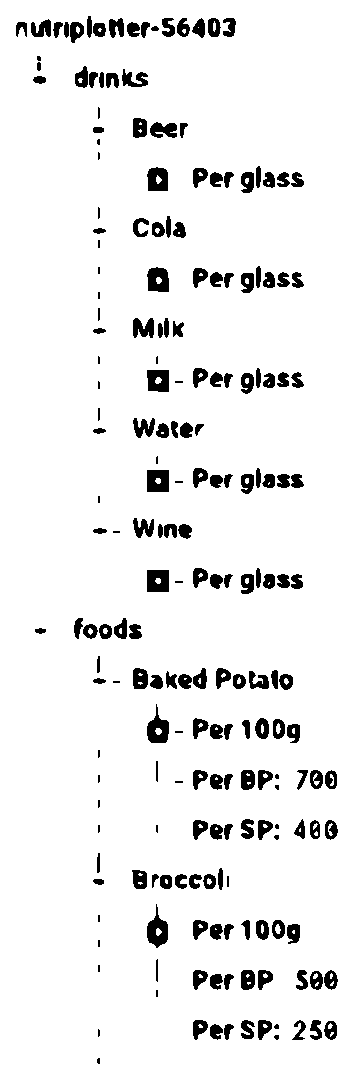
\includegraphics[width=0.15\textwidth]{figures/firebase.eps}
  \caption{Firebase Realtime Database schema.}
  \label{fig:firebase1}
\end{figure}
As Firebase operates with an asynchronous nature, it was quite challenging to handle the retrieval of information from the database and update the states of our code base accordingly. We tackled this issue by using async/wait statements in our code, in order to make sure that the function getting the data is always going to return a promise whilst also ensuring that it waits for the promise to settle and then to be returned, making sure that the state is updated and then used. We believe this was the best way to tackle the issue as we wanted the calculated nutritional data to be as precise and accurate as possible. 
Concluding in regards of using Firebase to include a database into our application, we believe if we were given the chance to go back and choose again we would have preferred an alternative database management system which would avoid duplication of data to save space and also would be more suitable for a larger database in case of further development of the application.\par
\subsubsection{Amplitude}
When it comes to creating an application, it is always useful to see the users behaviour with the app, in order to improve further. This is where analytics services become useful. Amplitude\cite{WEBSITE:amplitude} is one of the top analytics services out there, used by various very well known companies. Its successful compatibility with Expo, has given us the opportunity to gain insights into how users are using our app, which parts of the app they interact with, and what particular order of actions they take while using it. As seen in Figure 2, we have access to timestamps of each session. This could further be used to add/improve or delete any features in the future.\par
Overall, we believe Amplitude was a great addition to our application, with which the customer was very pleased and believed it would help them in future development and improvement of the app, in the case they hand it over to other developers.\par
\section{Quality Assurance}
\label{sec: quality assurance}
\subsection{Continuous Integration Issues}
\label{subsec: continuous integration issues}
We had ongoing issues with Gitlab's continuous integration pipeline, for a variety of reasons. The first was in generating key-pairs for setting up a runner for the pipeline itself. For an undiscovered reason, the lab machines we attempted to generate the keys from were generating empty key files when we tried to establish the runner at the start of the project. This was around the time of the ongoing issues with GitLab and the malware attack during the winter period, so the team believes that the initial problems we encountered may have been related to this. Although this predated the introduction of our unit testing, we were hopeful that we would have the pipeline functional before writing them so that we could add them relatively easy. As such, once the aforementioned issues were resolved, we got the pipeline to incorporate a runner for the tests that we planned to include. The pipeline itself worked as intended, but due to the issues discussed in the unit testing section of the dissertation, we were unable to effectively incorporate our tests into the CI pipeline since we could not have both the main application and unit testing on the same branch. This was unfortunate, as we already had a runner in place for the tests in our main repository which was made redundant by this development. We spent a large portion of time learning about the CI practises and were generally impressed by them, recognising the value that such a system would provide to the development of the project. For this reason, we were somewhat disappointed at not being able to get the pipeline as operational as hoped, but are glad of the opportunity we got to explore the benefits of it. Eventually, the decision to not incorporate the pipeline was made both due to time constraints and the issues that arose in testing.\par
\subsection{Unit Testing}
\label{subsec:unit testing}
Upon initially looking into testing, we expected the integration of testing to be relatively straightforward due to expo reportedly being configured for Jest\cite{WEBSITE:jest} testing - Jest being the Javascript testing framework largely relied upon by Facebook software engineers. We hoped to configure Jest using a preset for the Expo application (made by the Expo developers), but ran into trouble when attempting to do so. Jest and Expo are both rapidly-evolving libraries and so we were expecting we may run into issues with some of the recently-added components of the libraries. However, the issues we ran into were of compatibility between the Expo and Jest frameworks themselves. Many of the team attempted to configure Jest to work with Expo, but we had little success in getting it to work. Eventually, the unit tests were successfully configured to work with the branch they were a part of. This involved workarounds for a few known issues in the Jest library that we managed to trace. \par
However, due to a recent change in the library used to transpile the code for Jest, there were unresolvable method calls between the Jest and Expo libraries when trying to launch the Nutriplotter app itself as a result. We suspect this is a temporary compatibility issue between Jest and Expo, and it was observed while looking for fixes to the issue that the libraries are regularly updated and/or patched for issues of this kind. Frustratingly, we were unable to incorporate the testing onto our Master branch because of this issue. Many attempts were made to resolve the problem, and it was eventually decided to look for an alternative once the team was certain that a solution suitable for our purposes was unlikely. At the suggestion of our ASEP coach, we created a testing environment for the unit tests to be transferred to another repository. This bypassed the issue of the breaking change to the app's transpilation, as tests were entirely separated from the master version. Although this was a somewhat frustrating process, we were pleased that we managed to find a solution that would still incorporate unit testing. The majority of the bugs we discovered later arose as a result of the varying devices we used and almost invariably related to the screen size taking on an unexpected resolution. As such, we decided to provide greater weighting to our usability testing, which was conducted using a Google Form and a stable version of the application. We didn't provide our users with instructions on which type of device to use, largely because the more devices the app is tested on, the more likely we are to uncover display issues. \par
\subsection{Usability Testing}
\label{subsec:usability testing}
Our usability testing was conducted using the most recently published version of Nutriplotter and Google Forms. In the form, we included prompts outlining actions for the user to carry out. They were then asked to rate the ease with which they could do it, in addition to any further suggestions or comments regarding the feature in question. This was repeated for the key features of the app, such as the digital plate and the action of adding foods to the plate. The quantitative data was largely positive, showing that users were at worst ambivalent towards the application's design and navigation features in almost all cases. Mostly the Likert scales relating to design returned positive results from participants, and the drops in negative cases were often attributed to a bug that made itself apparent to the user. Users also seemingly found it easy to pick up how to use the app, judging by the responses to questions relating to it. The menu of the application was shown to be largely liked by users, although some reflected the wish to show more impact from option selections - such as a notification for when the "Restart" option is selected. Some jumpiness was also discovered in the adjustment of the plate segments for some plate sizes, which is an issue we were somewhat aware of and hope to fix before the conference demonstration for the client in late April. Conducting usability testing gave us an idea of the problems we would be likely to face when expanding Nutriplotter's audience to a wider group. It also helped to highlight a number of existing issues the team wasn't aware of, as well as better defining numerous issues that we were. We'd definitely incorporate usability testing again in the future, as it was extremely illuminating with regards to our key features, and provided an opportunity to test on a number of devices.\par
%------------------------------------------------------------------------------
\section{Deployment}
\label{sec: deployment}
\subsection{User Guide}
\label{subsec: user guide}
For best delivery to our customer, we created a step-by-step guide of our app, showing off every feature implemented, what each button and event does in the app, and how the pages navigate between them. We felt that it was necessary to provide the customer with the guide as there might be times where they might not be sure of what each object does on the app, and it would be best to have it all written down somewhere to avoid any confusion.\par
\subsection{User Manual}
The deployment process also included the development of a user manual for our application. This included documentation regarding the setup and installation of the environment using our source code from the repository, instructions on how to run the application on mobile devices, a guide on the structure of our source code for future development, a guide on how our database is set up and a few guidelines regarding our Wiki. This manual together with the detailed walkthrough of the app provided by the user guide mentioned in Section 8.1, we believe were an important part of a successful delivery of the product to the customer and will aid in solving minor issues they might face in the future.\par
\label{subsec: user manual}
\subsection{Final Product}
\label{subsec: Final Product}
At the end of the development phase, it was important to hand everything to our customer to ensure that they would be able to further develop the application in the case that they decided to do so. Our final product was delivered in a public GitHub repository, including an appropriate license, a README file with the right technical documentation required to set everything up and commented code. Moreover, the customer was given access rights as owner to both Firebase and Amplitude and was provided with both the user guide and manual with access rights to edit as required. The application was also published on Expo, with a barcode and a link to it, which we also provided the customer with.\par
Overall, we believe we've managed to successfully provide our customer with a functional and well-documented repository containing our progress within the given time frame and which is in a condition to aid future development. At the final demonstration, our customer was provided with everything, we thanked them for their cooperation throughout the entire process and for their help with supplying us with the right information. This was the end of us working on the project and a well-completed deployment.\par


%------------------------------------------------------------------------------
\section{Conclusions}
Upon completion of the Nutriplotter project, the team have had time to step back and reflect on the experience and knowledge gleaned from the project. The software practises we adopted ranged in their efficacy, but we were glad of the opportunities presented to test them in a real development context. We would likely adopt many of the practices again were we to repeat the project, and the experience gleaned from using them will likely help our individual development efforts in the future. In the scenario of repeating the project, we would likely incorporate other software process practices to help tackle certain areas of difficulty in the project. One such practice is the Question-Comment-Concern activity outlined in Michael Keeling's 'Design It!'\cite{Book:design_it}(Pg 298), This activity would have been useful at the outset of the project in order to bring all team members up to a suitable degree of Expo, Firebase and other new technologies via a structured method. Although we managed without this practice, we feel it could have helped to prevent some of the problems we ran into further down the track of development. The use of structured Use Cases, as exemplified in Hunt and Thomas' 'The Pragmatic Programmer'\cite{Book:pragprog}(Pg 206). Just as they were used in the book to help identify use cases for systems, the team believes that they would have provided a useful partner to our user cases, which we designed at the start of the design process. By using the thorough examination of potential functionality that use cases provide, they would hopefully give insights into areas of difficulty not yet considered by the team. This would allow us to sidestep some of the setbacks of development. Since one of our most significant setbacks was a divergence of design with the client, we consider this pertinent to our consideration of the project's overall success. Sufficient documentation for future developers was also a major aim throughout the project's lifecycle, particularly after the issues of poor readability were highlighted in Deimel and Naveda's project on the topic\cite{Book:deimel}, - introduced in the PSD course - which denotes some of the potential pitfalls poor documentation could lead future developers into. To avoid this, we put significant efforts into ensuring our developer docs were sufficient, and the fact that we could provide our user guide/manual combination is a point of pride now that development on the project is complete.\par 
We were extremely pleased that our client was seemingly impressed with the product we delivered after the final demonstration, particularly because we felt that we had a good relationship with the client throughout the project's duration and wanted to see Nutriplotter succeed. We're excited to be hopefully demonstrating it at the client's request on the floor of an upcoming conference in Glasgow focused on obesity. We initially chose Nutriplotter because we thought it would provide a suitable challenge for the team and were interested in the use of technology for innovating the recording of healthy eating. Our client's concept proved to be interesting but difficult to implement at times, and sometimes hard to define clearly. However, this was itself an informative experience, as the adaptive steps we had to take to remedy our missteps were good experience for adapting to client demands. Although it seemed difficult at the time, managing to realign our product idea with the client's idea was a situation we're likely to encounter in the future, and so learning from it now will likely be of use.\par


%==============================================================================
\bibliographystyle{unsrt}

\bibliography{dissertation}

\end{document}

%==============================================================================